% !TEX root = main.tex

\section{确定性规划}
% Closed world assumption
% STRIPS representation of actions
% STRIPS planning
% Relaxed plan heuristics

智能体应该能够对世界做出动作(action),而不仅仅是通过搜索解决问题或推理及知识表示。
核心是对动作的效果进行推理,并且计算什么动作能够达成特定的效果。

本节中主要关注确定性规划,即有完全的初始状态描述及确定性的动作效果。

\subsection{情景演算}
情景演算(Situation Calculation, SitCalc)三个基本部分
\begin{itemize}
	\item 动作(action):一组谓词
	\item 情景(situations):动作序列,$do(a,s)$为动作、情景到新情景的函数映射,$S_0$为初始情景
	\[do(put(a,b),do(put(b,c),S_0))\]
	要区别情景与状态(state),如将硬币转两次,情景/动作历史不同,但状态都是一样的
	\item 流(fluent):从情景到情景的谓词或函数(动态变化过程),用谓词或函数符号描述,其中最后一个参数为情景,如$Holding(r,x,s)$代表机器人$r$在状态$s$下拿着物体$x$,有
	\[\lnot Holding(r,x,s)\land Holding(r,x,do(pickup(r,x),s))\]
	经过后面的流操作会得到一个新情景下的谓词
	\item 条件(precondition):动作执行的前提条件
	\item 影响(effect):执行动作后改变的流。 % the fluents that change as the result of performing the action
	如下在情景$s$下执行修复动作后,$x$就不是破碎的
	\[\lnot Broken(x,do(repair(r,x)),s)\]
\end{itemize}

情景演算的形式化仅陈述了执行动作的影响,而没有阐述没影响的部分。
但是给定一个流只有很少的动作会被影响,而大多数都保持不变。

形式化后的情景即可以利用归结进行规划,但是开销会非常大。
而框架(frame)问题则是找到一种高效的方法来确定动作的非效果(non-effects)。而不是显式地将它们全部写下来,可以考虑用一阶逻辑。

\subsection{STRIPS}
传统的规划没有不完全或不确定的信息,因此可以做以下假设。
\begin{itemize}
	\item 封闭世界假设(Closed-World Assumption, CWA):初始状态的信息是完备的,用于表示世界状态的知识库是一系列真实的原子事实(与数据库类似)。
	如$emp(A,C)$不在数据库中,则$\lnot emp(A,C)$为真。
	\item 动作的前提只能是原子命题的合取
	\item 动作的影响只会使原子命题变真或变假,不会出现条件影响或析取影响
\end{itemize}

STRIPS(Stanford Research Institute Problem Solver):
\begin{itemize}
	\item 世界被表示成封建世界知识库(CW-KB),一个STRIPS的动作表示成更新CW-KB的方式
	\item 一个动作生成新的KB,用以描述新的世界
\end{itemize}

在SitCalc中我们可能有不完全的信息(用一阶逻辑公式表示),而在STRIPS中,我们有完整的信息(用CW-KB表示)。

STRIPS中需要用3个列表来表示一个动作
\begin{itemize}
	\item 动作的前提\verb'pre'
	\item 动作增加的影响\verb'add'
	\item 动作减少的影响\verb'delete'
\end{itemize}
\begin{example}
$pickup(X)$:
\begin{itemize}
\item $Pre: {handempty, clear(X), ontable(X)}$
\item $Adds: {holding(X)}$
\item $Dels: {handempty, clear(X), ontable(X)}$
\end{itemize}
\end{example}

注意STRIPS的表达力还是有限制的,如它没有条件(conditional)影响。
因此需要有表达力更强的语言Action Description Language(ADL),允许在前提中有任意公式,而且可以有条件和全称影响。

可以将规划看成是一个搜索问题,每个动作都是由一个CW-KB到CW-KB的映射,但搜索空间会非常巨大。

\subsection{松弛问题}
传统的规划给出
\begin{itemize}
	\item 一个封闭世界知识库表示原始状态
	\item 一组STRIPS动作(从状态到新状态的映射)
	\item 一个目标状态
\end{itemize}

放松(relaxed)问题即考虑\textbf{忽略删除动作}的列表,这样可能得到有用的启发式函数估计。

\begin{theorem}
放松问题的一个最优规划的长度是原始问题最优规划长度的下界
\end{theorem}
\begin{proof}
由于我们将所有影响都添加了,并且不删除负面影响,因此很直觉地会很快得到目标。
令$P$为原始问题,$P'$为放松问题,我们希望得到$Sols(P)\subset Sols(P')$,则有$Minlen(Sols(P'))\leq Minlen(Sols(P))$。
\begin{itemize}
\item 令$a_0,\ldots,a_{n-1}$为$P$的解,证明它也是$P'$的一个解。
令$s_0$为初始状态,令$s_{i+1}=s_i\cup add(a_i)-del(a_i),\forall i<n$,且$Goal\subset s_n$,$pre(a_i)\subset s_i,\forall i < n$。
\item 又令$s_0'=s_0$,且$s_{i+1}'=s_i'\cup add(a_i)$,通过数学归纳法证明$s_i\subset s_i',\forall i \leq n$。
\begin{itemize}
	\item 归纳奠基:$i=0$时$s_0\subset s_0'=s_0$
	\item 归纳假设:假设$s_i\subset s_i',\forall i<n$,证明$s_{i+1}\subset s_{i+1}'$
	\item 推理:因为$a_i$在$s_i$中是可采纳的,即$pre(a_i)\subset s_i$,因此$pre(a_i)\subset s_i\subset s_i'$,即$a_i$在$s_i'$中是可采纳的。所以得到
	\[s_{i+1}=s_i\cup add(a_i)-del(a_i)\subset s_i'\cup add(a_i)=s_{i+1}'\]
\end{itemize}
\end{itemize}
进而$Goal\subset s_n\subset s_n'$,且$pre(a_i)\subset s_i\subset s_i',\forall i<n$,因此$a_0,\ldots,a_{n-1}$也是$P'$的一个解。
\end{proof}

因此最优放松问题的规划可以作为$A^\star$算法的可采纳启发式函数。
然而在放松问题中计算一个最优的问题是NP难的,可以从$S$开始建立层次(layered)结构使其到达目标。

可达性分析:$s_0,a_1,s_1,\ldots,a_n,s_n$,直到$s_n\subset Goal$,或者状态层$s_n$不再改变(到达不动点)。
\textemph{注意动作层的计算一定要小心是否漏动作}。
\begin{proposition}
令$a_0,\ldots,a_{n-1}$为$S_0$中可采纳的动作序列,令$s_0=S_0$,且$s_{i+1}=s_i\cup add(a_i)-del(a_i)$。
那么$\forall i<n,\exists j,k\leq i$使得$a_i\in A_k$且$s_i\subset S_j$
\end{proposition}
\begin{analysis}
用数学归纳法
\begin{itemize}
	\item 归纳奠基:$i=0$显然成立
	\item 归纳假设:假设$\forall i <n \exists j\leq i:\;s_i\subset S_j$
	\item 因为$pre(a_i)\subset s_i,pre(a_i)\subset S_j$,令$k$为最小的$u\leq j$使得$pre(a_i)\subset S_u$,那么$a_i\in A_k$,故$add(a_i)\subset S_{k+1}\subset S_{j+1}$
	因此
	\[s_{i+1}\subset s_i\cup add(a_i)\subset S_j\cup S_{j+1}=S_{j+1}\]
\end{itemize}
\end{analysis}

\begin{theorem}
假设状态层不再改变且目标不被满足,则原始规划问题是不可解的。
\end{theorem}
\begin{proof}
用反证法,假设$a_0,\ldots,a_{n-1}$为原始问题的一个解,则$Goal\subset s_n$。
由前面的命题,存在$m\leq n$使得$Goal\subset s_n\subset S_m$,导致矛盾。
\end{proof}

假设目标$G$包含在状态层中,现在想要计算一个好的放松规划,想法即对每个$i$选择最小的$A_i$子集。
\begin{figure}[H]
\centering
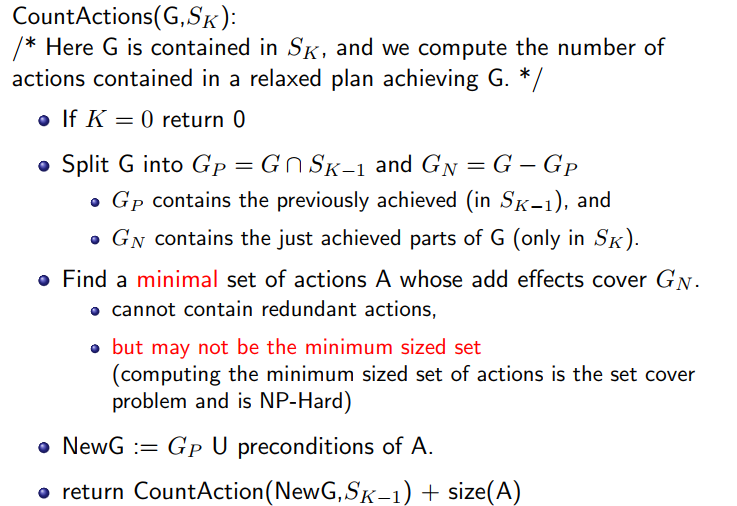
\includegraphics[width=0.8\linewidth]{fig/count_actions.png}
\end{figure}
进而变成一个集合覆盖问题:从集合的集合$S$中选择$m$个集合使得其并集可以覆盖全集。

CountActions从最后一层往前迭代,将目标$G$划分为$G_P$和$G_N$。
\[\begin{aligned}
G_P&=G\cap S_{K-1}\\
G_N&=G-G_P\\
A&=\text{影响成为}G_N\text{的最小覆盖}\\
NewG&=G_P\cup A\text{的前提}
\end{aligned}\]

\begin{theorem}
假设$Goal\subset S_k$,对于$i<k$,令$A_{i-1}'$为调用CountActions($G_i,S_i$)的结果,则$A_0',\ldots,A_{k-1}'$为松弛问题的一个解。
\end{theorem}
\begin{proof}
用数学归纳法
% TODO
\end{proof}